% !TEX program = xelatex
% !TEX TS-program = xelatex
% ---------------------------------------------------------------
% 本文含中文，必须使用 XeLaTeX（或 LuaLaTeX）编译。
% 用 pdfLaTeX 编译会报：CTeX fontset `mac' is unavailable in current mode
% 命令行编译：latexmk DiffusionM.tex   （.latexmkrc 已设 $pdf_mode = 5）
%
% 图片素材：images/ 下是原图，images/gen/ 是排版用的派生图
%   cat_white / cat_black / cat_mix : 三只猫（缩放版）
%   gpt_2to1                        : GPT 生图（裁成 2:1）
%   cat_noise1 / cat_noise2         : 白猫叠加高斯噪声（加噪 1 次 / 2 次）
%   noise_gray                      : 纯高斯噪声（x_T，也用作箭头上的噪声图块）
% ---------------------------------------------------------------
\RequirePackage{iftex}
\ifPDFTeX
  \errmessage{This document must be compiled with XeLaTeX (Chinese fontset is unavailable under pdfLaTeX). Please run: latexmk -xelatex DiffusionM.tex}
  \endinput
\fi

\documentclass[UTF8,a4paper,12pt]{ctexart}

\usepackage{amsmath}
\numberwithin{equation}{section}
\usepackage{amssymb}
\usepackage{bm}
\usepackage{graphicx}
\graphicspath{{images/}{images/gen/}}
\usepackage{float}
\usepackage{caption}
\captionsetup{font=small,labelfont=normalfont,labelsep=colon,skip=5pt}
\usepackage{tikz}
\usetikzlibrary{arrows.meta,positioning,calc,fit,backgrounds,shapes.misc}
\usepackage{fancyhdr}
\pagestyle{fancy}
\fancyhf{}
\fancyhead[R]{\thepage}
\renewcommand{\headrulewidth}{0pt}
\setlength{\headheight}{15pt}
\fancypagestyle{plain}{
\fancyhf{}
\fancyhead[R]{\thepage}
\renewcommand{\headrulewidth}{0pt}
}

\renewcommand{\topfraction}{0.9}
\renewcommand{\bottomfraction}{0.7}
\renewcommand{\textfraction}{0.1}
\renewcommand{\floatpagefraction}{0.8}

% 公式上下间距：必须放在 \AtBeginDocument 里，否则会被 \document
% 开头的 \normalsize 重置回类默认值（12pt），设了等于白设。
\AtBeginDocument{%
  \setlength{\abovedisplayskip}{16pt plus 3pt minus 5pt}%
  \setlength{\belowdisplayskip}{16pt plus 3pt minus 5pt}%
  \setlength{\abovedisplayshortskip}{8pt plus 2pt minus 2pt}%
  \setlength{\belowdisplayshortskip}{8pt plus 2pt minus 2pt}%
  \setlength{\jot}{6pt}%  align 等多行公式行间距（默认 3pt）
}
\setlength{\textfloatsep}{8pt plus 2pt minus 2pt}
\setlength{\intextsep}{8pt plus 2pt minus 2pt}
\setlength{\abovecaptionskip}{4pt}

\usepackage{xcolor}
\usepackage[colorlinks=true,linkcolor=black,urlcolor=blue,citecolor=black]{hyperref}

\title{Diffusion Model}
\date{2026年9月23日}

% ---- 插图里反复用到的样式 ----
\tikzset{
  flowbox/.style={rounded corners=4pt, draw=blue!55!black, fill=blue!7,
                  inner sep=3pt, align=center, font=\small},
  flowarr/.style={-{Stealth[length=1.8mm,width=1.2mm]}, draw=gray!75, line width=0.7pt},
  flowlab/.style={font=\small, text=black!85, align=center},
  thumb/.style={inner sep=0pt, outer sep=0pt},
}
% 在 (#1,#2) 附近随机撒 #3 个噪点的辅助命令（#4 为随机种子）
\newcommand{\noisedots}[4]{%
  \pgfmathsetseed{#4}%
  \foreach \k in {1,...,#3}{%
    \pgfmathsetmacro{\dx}{0.56*rand}%
    \pgfmathsetmacro{\dy}{0.56*rand}%
    \fill[black!78] (#1+\dx,#2+\dy) circle (0.5pt);%
  }%
}

\begin{document}

\maketitle

\section{引言}

在很长一段时间里，我对 AI 生图的印象还停留在``风格化渲染''上：给模型一张照片，它返回一张动漫风格的图。直到 GPT 2.0 系列模型出现，这个印象才被彻底打破——它生成的 90 年代中国家庭照片逼真得令人惊讶，构图、光线乃至老照片特有的质感都恰到好处（图~\ref{fig:gpt}）。

\begin{figure}[htbp]
\centering
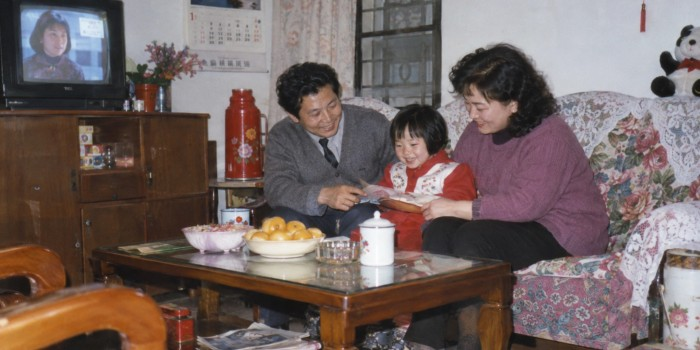
\includegraphics[width=5.76cm]{gpt_2to1}
\caption{AI生图示例}
\label{fig:gpt}
\end{figure}

于是我开始认真了解图像生成这个方向，很快发现一个名字反复出现：Diffusion Model。今天图像生成领域的主流工作几乎都建立在它之上；而在机器人学习领域，也有一批颇有影响力的工作（例如 Diffusion Policy）以它为骨架。市面上有很多关于扩散模型的博客与视频，但是他们大多都有些复杂亦或是不够直观，于是我就想尝试写一篇关于扩散模型的博客，以便日后在自己忘记相关知识时回头看能再次捡起。

本文主要梳理了扩散模型的基本思想，并尝试完整推导 DDPM 的训练目标与采样过程，侧重于直观理解，省略了部分纯计算性的细节，并在其中附上了笔者自己的理解，如有错误，还请指正；整体框架参考了李宏毅《机器学习》2023 春季课程中扩散模型的相关章节。

\section{基本概念}

先从一个形象的例子开始。和所有机器学习方法一样，扩散模型方法无法输出它从未见过的样本：训练时需要一批真实图像，最终生成的也只是无限逼近这批样本。比如用一批猫的照片训练，模型就生成不出狗，而只能生成猫，或者猫的组合——这里说的组合是指：比如用白猫与黑猫的照片训练后，模型可以生成一只头像白色、身子纯黑的猫，如图~\ref{fig:cats} 所示。当然现在网上已经有很多这样的组合，比如将某些明星 P 图在饮料上亦或是将某些动漫卡通图像从它原本的形态生成一张青蛙形态的照片。

\begin{figure}[htbp]
\centering
\begin{minipage}[t]{4.11cm}\centering
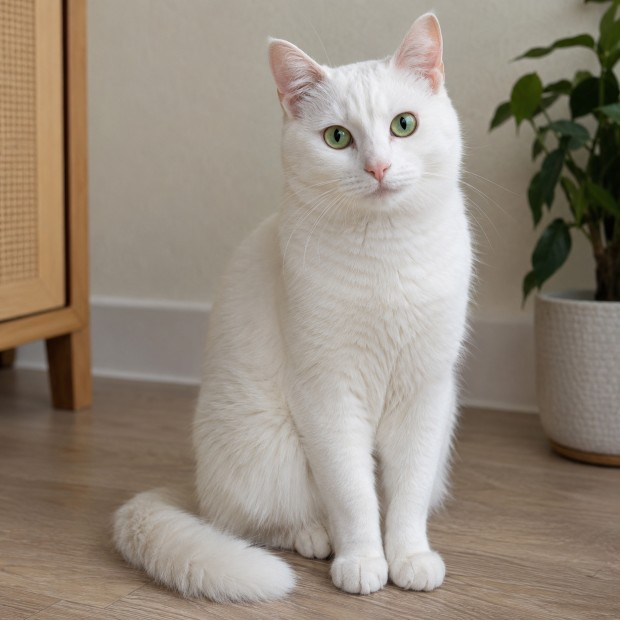
\includegraphics[width=0.84\linewidth]{cat_white}\\[1pt]
{\small 白猫}
\end{minipage}\hfill
\begin{minipage}[t]{4.11cm}\centering
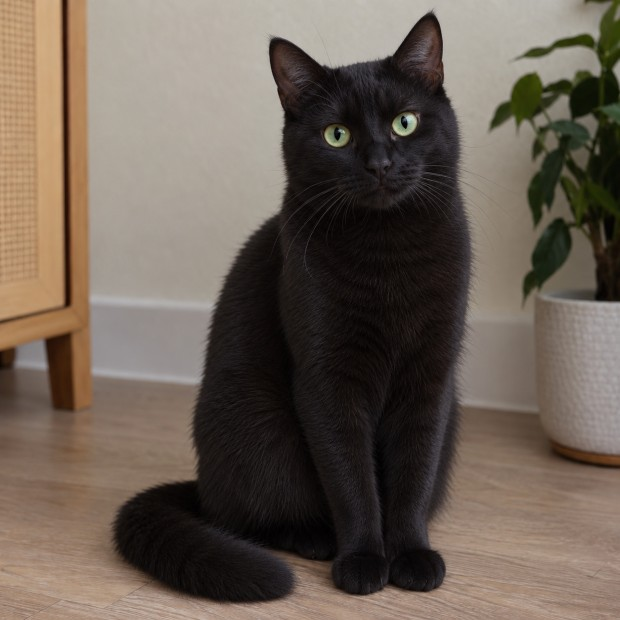
\includegraphics[width=0.84\linewidth]{cat_black}\\[1pt]
{\small 黑猫}
\end{minipage}\hfill
\begin{minipage}[t]{4.11cm}\centering
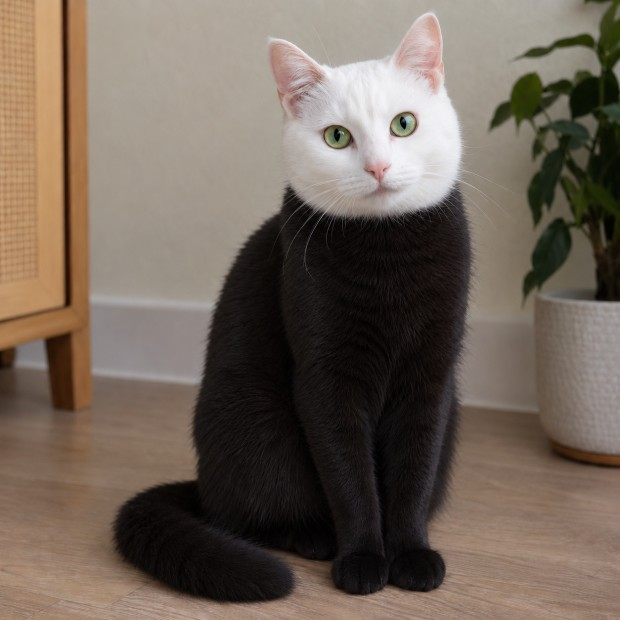
\includegraphics[width=0.84\linewidth]{cat_mix}\\[1pt]
{\small 合成猫}
\end{minipage}
\caption{训练与生成}
\label{fig:cats}
\end{figure}

扩散模型可以拆成方向相反的两条链：前向过程往真实图片里不断加入噪声，直到它接近标准高斯噪声；反向过程反过来走，从随机噪声出发一步步去除之前加入的噪声，最终恢复出图片。

两条链的流程分别如图~\ref{fig:forward_chain} 与图~\ref{fig:reverse_chain}所示。加噪链上，每一步都在当前照片上叠加一次高斯噪声（箭头上方的噪声图块就是这一步加入的 $\bm{\epsilon}$），加噪 $n$ 次之后照片变成一片纯噪声 $\bm{x}_T$；去噪链则把同一组照片倒过来走，每一步都由网络预测当前混入的噪声、再减掉一部分，去噪 $n$ 次之后恢复出干净的 $\bm{x}_0$。

\begin{figure}[H]
\centering
\resizebox{0.95\textwidth}{!}{%
\begin{tikzpicture}[x=1cm,y=1cm]
\node[thumb] (A) at (0,0) {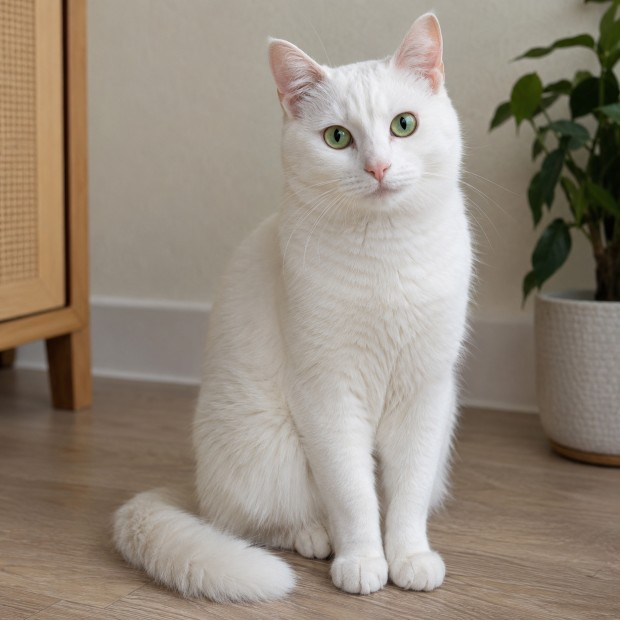
\includegraphics[width=1.96cm]{cat_white}};
\node[thumb] (B) at (4.2,0) {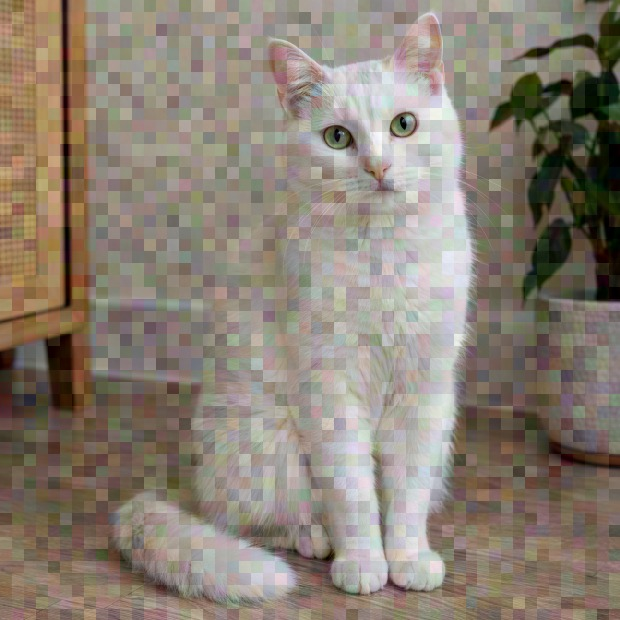
\includegraphics[width=1.96cm]{cat_noise1}};
\node[thumb] (C) at (8.4,0) {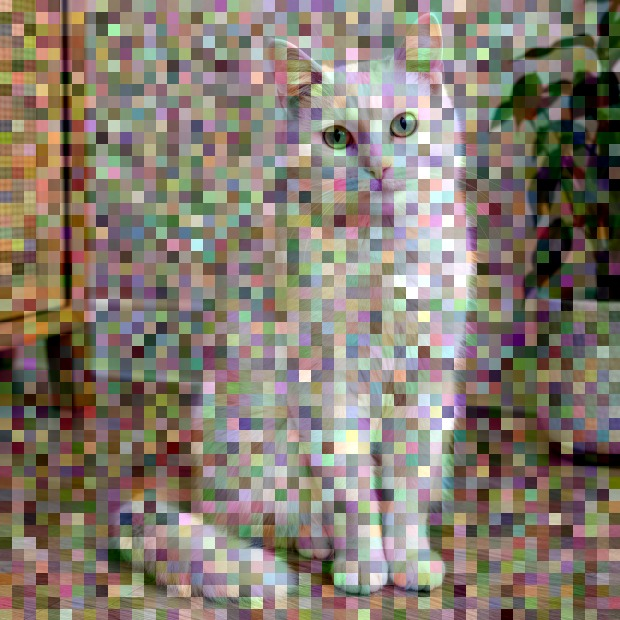
\includegraphics[width=1.96cm]{cat_noise2}};
\node[thumb] (D) at (12.6,0) {
\includegraphics[width=1.96cm]{noise_gray}};
\draw[flowarr] ($(A.east)+(0.04,0)$) -- ($(B.west)+(-0.04,0)$);
\draw[flowarr] ($(B.east)+(0.04,0)$) -- ($(C.west)+(-0.04,0)$);
\draw[flowarr] ($(C.east)+(0.04,0)$) -- (10.1,0);
\node[flowlab] at (10.5,0) {$\cdots$};
\draw[flowarr] (10.9,0) -- ($(D.west)+(-0.04,0)$);
\foreach \x in {2.1,6.3,10.5}{%
  \node[thumb] at (\x,0.62) {
\includegraphics[width=1.15cm,height=0.68cm]{noise_gray}};
  \node[flowlab] at (\x,1.2) {$+\bm{\epsilon}$};
}
\node[flowlab, below=4pt of A] {$\bm{x}_0$（白猫）};
\node[flowlab, below=4pt of B] {加噪 1 次};
\node[flowlab, below=4pt of C] {加噪 2 次};
\node[flowlab, below=4pt of D] {加噪 $n$ 次\\$\bm{x}_T$（纯噪声）};
\end{tikzpicture}}
\caption{前向加噪流程}
\label{fig:forward_chain}
\end{figure}

\begin{figure}[H]
\centering
\resizebox{0.95\textwidth}{!}{%
\begin{tikzpicture}[x=1cm,y=1cm]
\node[thumb] (A) at (0,0) {
\includegraphics[width=1.96cm]{noise_gray}};
\node[thumb] (B) at (4.6,0) {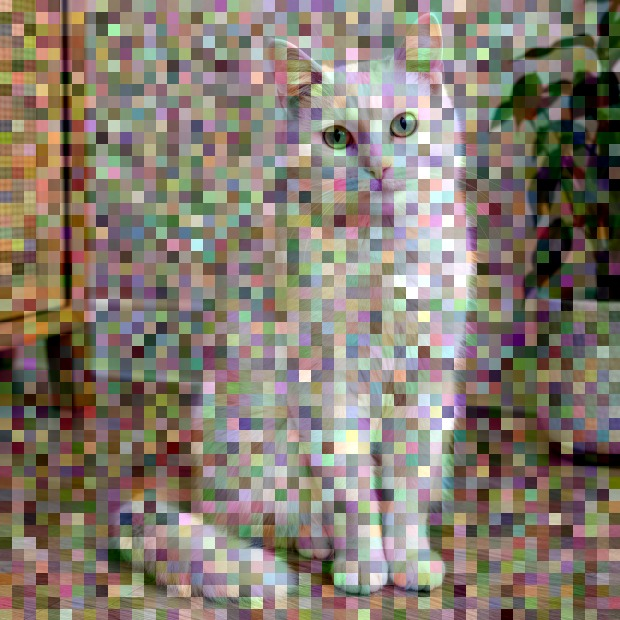
\includegraphics[width=1.96cm]{cat_noise2}};
\node[thumb] (C) at (9.2,0) {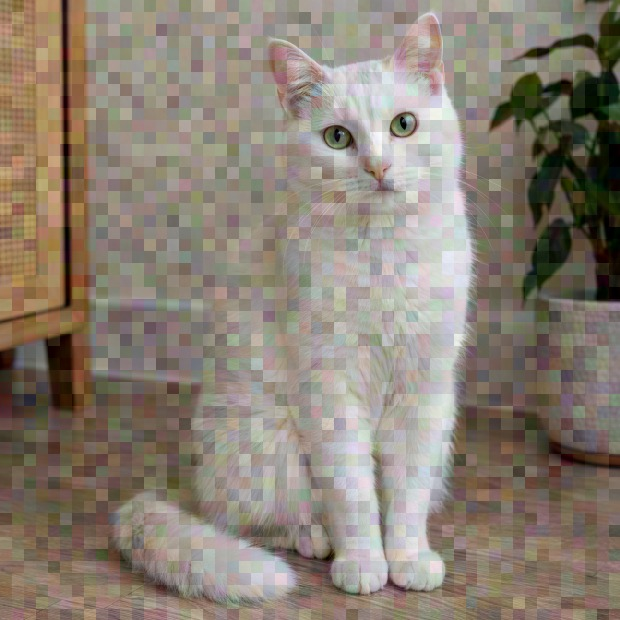
\includegraphics[width=1.96cm]{cat_noise1}};
\node[thumb] (D) at (13.8,0) {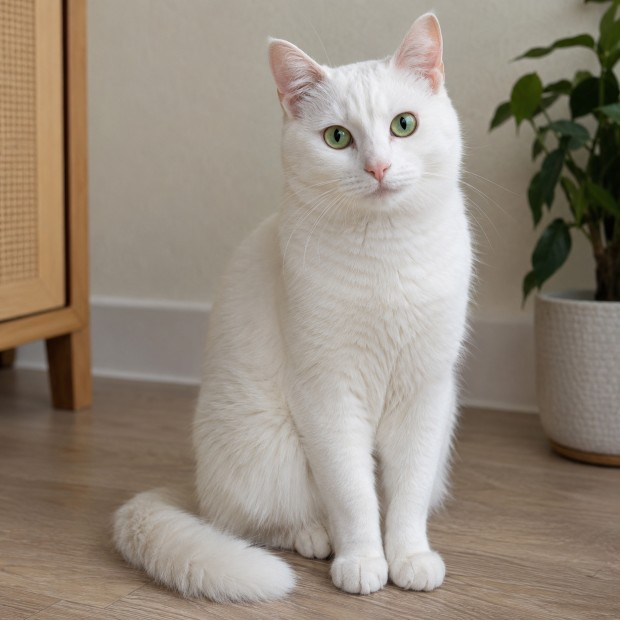
\includegraphics[width=1.96cm]{cat_white}};
\draw[flowarr] ($(A.east)+(0.04,0)$) -- ($(B.west)+(-0.04,0)$);
\draw[flowarr] ($(B.east)+(0.04,0)$) -- ($(C.west)+(-0.04,0)$);
\draw[flowarr] ($(C.east)+(0.04,0)$) -- (11.4,0);
\node[flowlab] at (11.7,0) {$\cdots$};
\draw[flowarr] (12.0,0) -- ($(D.west)+(-0.04,0)$);
\foreach \x in {2.3,6.9,11.5}{%
  \node[flowbox, minimum width=2.35cm, minimum height=1.0cm] at (\x,1.15)
    {网络预测\\并去除噪声};
  \draw[flowarr] (\x,0.6) -- (\x,0.12);
}
\node[flowlab, below=4pt of A] {$\bm{x}_T$（纯噪声）};
\node[flowlab, below=4pt of B] {去噪 1 次};
\node[flowlab, below=4pt of C] {去噪 2 次};
\node[flowlab, below=4pt of D] {去噪 $n$ 次\\$\bm{x}_0$（白猫）};
\end{tikzpicture}}
\caption{反向去噪流程}
\label{fig:reverse_chain}
\end{figure}

这个过程很像还原一个魔方：前向过程是人为地把一个六面同色的标准魔方一步步打乱，直到六个面全都乱掉；反向过程则是沿相反的轨迹把它拧回去，直到恢复成标准魔方。当然，现实中的魔方有现成公式可循，以及现实生活中我们的标准状态并非是六面同色的状态，比如现在有很多博主尝试用多个魔法去画心形亦或是其他图形。但这里关心的不是公式，而是让模型记住我们想要的``标准状态''是什么，再把打乱后的魔方交还给它去复原回去。

\begin{figure}[htbp]
\centering
\begin{tikzpicture}[x=1cm,y=1cm]
\node[flowbox, minimum width=2.3cm, minimum height=1.0cm] (x0) at (0,0)
  {$\bm{x}_0$\\真实数据};
\node[flowbox, minimum width=2.3cm, minimum height=1.0cm] (xt) at (4.6,0)
  {$\bm{x}_t$\\带噪数据};
\node[flowbox, minimum width=2.3cm, minimum height=1.0cm] (xT) at (9.2,0)
  {$\bm{x}_T$\\近似纯噪声};
\draw[flowarr] ($(x0.east)+(0.05,0)$) -- node[above,font=\small]{逐步加噪} ($(xt.west)+(-0.05,0)$);
\draw[flowarr] ($(xt.east)+(0.05,0)$) -- node[above,font=\small]{逐步加噪} ($(xT.west)+(-0.05,0)$);
\draw[flowarr] ($(xT.south)+(0,-0.05)$) .. controls +(0,-0.85) and +(0,-0.85) .. ($(xt.south)+(0,-0.05)$);
\node[flowlab] at (6.9,-0.72) {学习去噪};
\draw[flowarr] ($(xt.south)+(0,-0.05)$) .. controls +(0,-0.85) and +(0,-0.85) .. ($(x0.south)+(0,-0.05)$);
\node[flowlab] at (2.3,-0.72) {学习去噪};
\node[flowlab] at (4.6,-1.75) {生成方向：从噪声出发，逐步恢复结构};
\end{tikzpicture}
\caption{前向与反向}
\label{fig:flow}
\end{figure}

\section{前向加噪}

\subsection{单步加噪}

设有一张干净、清晰的图片作为初始样本，记为 $\bm{x}_0$。前向过程规定了一条固定的马尔可夫链：每一步只在当前图片上叠一点点高斯噪声，加多少由系数 $\beta_t\in(0,1)$ 决定。$\bm{x}_t$、$\bm{x}_{t-1}$ 与这一步加入的噪声 $\bm{\epsilon}_t$ 之间的关系式就是
\begin{equation}\label{eq:3.1}
\bm{x}_t=\sqrt{1-\beta_t}\,\bm{x}_{t-1}+\sqrt{\beta_t}\,\bm{\epsilon}_t,
\qquad \bm{\epsilon}_t\sim\mathcal{N}(\bm{0},\bm{I}).
\end{equation}
换句话说，在给定 $\bm{x}_{t-1}$ 时，$\bm{x}_t$ 服从一个均值为 $\sqrt{1-\beta_t}\,\bm{x}_{t-1}$、方差为 $\beta_t\bm{I}$ 的高斯分布：
\begin{equation}\label{eq:3.2}
q(\bm{x}_t\mid\bm{x}_{t-1})
=\mathcal{N}\!\left(\sqrt{1-\beta_t}\,\bm{x}_{t-1},\,\beta_t\bm{I}\right),
\qquad t=1,2,\ldots,T.
\end{equation}

其中 $\beta_t$ 是第 $t$ 步的噪声强度，它随着 $t$ 的增大而增大：也就是说，随着噪声不断加入，图像里噪声的占比越来越大、原来真实图像的占比越来越小，直到最终的 $\bm{x}_T$ 中几乎全部都是噪声。这两个系数的取法可以严格说清楚，出发点只有一条：让加噪之后样本的边缘方差保持不变。为此需要一条关于高斯的基本结论：若 $X\sim\mathcal{N}(\mu_1,\sigma_1^2)$ 与 $Y\sim\mathcal{N}(\mu_2,\sigma_2^2)$ 相互独立，则它们的加权和仍是高斯，且
\begin{equation}\label{eq:3.3}
aX+bY\sim\mathcal{N}\!\left(a\mu_1+b\mu_2,\;a^2\sigma_1^2+b^2\sigma_2^2\right).
\end{equation}
从定义可以直接验证：期望按线性叠加，是 $a\mu_1+b\mu_2$；方差为 $a^2\sigma_1^2+b^2\sigma_2^2+2ab\,\mathrm{Cov}(X,Y)$，独立性使协方差项恰好为零（从密度的角度看，这等价于两个高斯密度做卷积，而卷积结果仍是高斯密度）。

把式~\eqref{eq:3.3} 用在式~\eqref{eq:3.1} 上（取 $a=\sqrt{1-\beta_t}$、$b=\sqrt{\beta_t}$，两个噪声项均值为零、方差为 $1$），得到 $\bm{x}_t$ 的边缘方差：
\begin{equation}\label{eq:3.4}
\mathrm{Var}(\bm{x}_t)=(1-\beta_t)\,\mathrm{Var}(\bm{x}_{t-1})+\beta_t .
\end{equation}
这是一个把方差往 $1$ 收拢的不动点迭代：若 $\mathrm{Var}(\bm{x}_{t-1})=1$，则 $\mathrm{Var}(\bm{x}_t)=1$；方差偏大就被压小，偏小就被抬大。因此只要初始数据做过标准化（实际训练正是如此），整条链上每一步的边缘方差都严格等于 $1$，加噪再多也不会尺度爆炸或塌缩。顺带这也解释了根号从哪里来：方差里的贡献是系数的平方，要让旧内容的方差贡献恰好乘 $(1-\beta_t)$、新噪声恰好贡献 $\beta_t$，两个系数就必须开根号；若均值系数直接写成 $1-\beta_t$，方差会按 $(1-\beta_t)^2$ 衰减，几十步后样本尺度就塌掉了。单步的 $\beta_t$ 通常很小（例如从 $10^{-4}$ 线性增长到 $0.02$），所以单看一步几乎看不出变化——这正是“扩散”这个名字的由来：像一滴墨在清水里慢慢散开。

\subsection{一步到位}

实际操作中，并不会真的一步一步加 $t$ 次噪声：既然每一步的关系都已知，就可以把式~\eqref{eq:3.1} 逐层代入，直接推出 $\bm{x}_t$ 与 $\bm{x}_0$ 的关系，让整个前向加噪等效成一步。记
\begin{equation}\label{eq:3.5}
\alpha_t=1-\beta_t,\qquad
\bar{\alpha}_t=\prod_{s=1}^{t}\alpha_s .
\end{equation}
以两步为例，把式~\eqref{eq:3.1} 代入自身：
\begin{align}
\bm{x}_2&=\sqrt{\alpha_2}\,\bm{x}_1+\sqrt{1-\alpha_2}\,\bm{\epsilon}_2\notag\\[-2pt]
&=\sqrt{\alpha_1\alpha_2}\,\bm{x}_0
+\underbrace{\sqrt{\alpha_2(1-\alpha_1)}\,\bm{\epsilon}_1
+\sqrt{1-\alpha_2}\,\bm{\epsilon}_2}_{\text{两个独立高斯的加和}} .
\label{eq:3.6}
\end{align}
关键就在最后这一项：它把两次加入的噪声合到了一起。直接套用式~\eqref{eq:3.3}——两个噪声相互独立、均值都是零，系数为 $a=\sqrt{\alpha_2(1-\alpha_1)}$ 与 $b=\sqrt{1-\alpha_2}$，于是加和的均值为零、方差按系数平方累加：
\begin{equation}\label{eq:3.7}
\sqrt{\alpha_2(1-\alpha_1)}\,\bm{\epsilon}_1+\sqrt{1-\alpha_2}\,\bm{\epsilon}_2
\sim\mathcal{N}\Bigl(\bm{0},
\underbrace{\bigl[\alpha_2(1-\alpha_1)+(1-\alpha_2)\bigr]}_{=\,1-\alpha_1\alpha_2\,=\,1-\bar{\alpha}_2}\bm{I}\Bigr),
\end{equation}
所以这两个噪声可以等效成一个标准形式的高斯，记作 $\bm{\epsilon}\sim\mathcal{N}(\bm{0},\bm{I})$。照此规律归纳到任意 $t$ 步，就得到从 $\bm{x}_0$ 直接跳到任意时刻的闭式：
\begin{equation}\label{eq:3.8}
\bm{x}_t=\sqrt{\bar{\alpha}_t}\,\bm{x}_0+\sqrt{1-\bar{\alpha}_t}\,\bm{\epsilon},
\qquad \bm{\epsilon}\sim\mathcal{N}(\bm{0},\bm{I}).
\end{equation}
也就是说，前面 $t$ 次分别加入的噪声，合起来等效为一个方差为 $1-\bar{\alpha}_t$ 的高斯噪声；$\bar{\alpha}_t$ 随 $t$ 单调减小，噪声的等效占比就越来越大，直到 $t=T$ 时 $\bm{x}_T$ 近似纯噪声。

关于 $\beta_t$ 该怎么取：取太小，$T$ 必须很大、采样很慢；取太大，单步破坏的信息过多、反向过程更难学。常见做法是让 $\beta_t$ 从 $10^{-4}$ 到 $0.02$ 线性增长，或者采用余弦形式的调度。

\begin{figure}[htbp]
\centering
\begin{tikzpicture}[x=1cm,y=1cm]
\node[draw=black!70, line width=0.5pt, minimum size=1.3cm, inner sep=0pt]
  (b0) at (0,0) {\fontsize{17}{17}\selectfont 猫};
\node[draw=black!70, line width=0.5pt, minimum size=1.3cm, inner sep=0pt]
  (b1) at (2.75,0) {\fontsize{17}{17}\selectfont 猫};
\node[draw=black!70, line width=0.5pt, minimum size=1.3cm, inner sep=0pt]
  (b2) at (5.5,0) {\fontsize{17}{17}\selectfont 猫};
\node[draw=black!70, line width=0.5pt, minimum size=1.3cm, inner sep=0pt]
  (b3) at (8.25,0) {\fontsize{17}{17}\selectfont 猫};
\node[draw=black!70, line width=0.5pt, minimum size=1.3cm, inner sep=0pt]
  (b4) at (11,0) {};
\noisedots{2.75}{0}{45}{21}
\noisedots{5.5}{0}{90}{32}
\noisedots{8.25}{0}{160}{43}
\noisedots{11}{0}{330}{54}
\draw[flowarr] ($(b0.east)+(0.04,0)$) -- ($(b1.west)+(-0.04,0)$);
\draw[flowarr] ($(b1.east)+(0.04,0)$) -- ($(b2.west)+(-0.04,0)$);
\draw[flowarr] ($(b2.east)+(0.04,0)$) -- ($(b3.west)+(-0.04,0)$);
\draw[flowarr] ($(b3.east)+(0.04,0)$) -- ($(b4.west)+(-0.04,0)$);
\foreach \x in {1.375,4.125,6.875,9.625}{%
  \node[flowlab] at (\x,0.95) {$+\bm{\epsilon}$};
}
\node[flowlab, below=3pt of b0] {$\bm{x}_0$};
\node[flowlab, below=3pt of b1] {$\bm{x}_1$};
\node[flowlab, below=3pt of b2] {$\cdots$};
\node[flowlab, below=3pt of b3] {$\bm{x}_{T-1}$};
\node[flowlab, below=3pt of b4] {$\bm{x}_T$};
\end{tikzpicture}
\caption{前向加噪示意}
\label{fig:noise_chain}
\end{figure}

\section{反向去噪}

\subsection{单步去噪}

生成时手里只有 $\bm{x}_T\sim\mathcal{N}(\bm{0},\bm{I})$，希望一步步退回 $\bm{x}_0$。反向过程同样是一条马尔可夫链，它的每一步是条件分布 $q(\bm{x}_{t-1}\mid\bm{x}_t)$，直观上回答的问题是：拿到一张加了 $t$ 次噪声的图片，它少加一次噪声时最可能长什么样？

按贝叶斯公式把它展开，
\begin{equation}\label{eq:4.1}
q(\bm{x}_{t-1}\mid\bm{x}_t)=\frac{q(\bm{x}_{t-1})\,q(\bm{x}_t\mid\bm{x}_{t-1})}{q(\bm{x}_t)} .
\end{equation}
分子里的 $q(\bm{x}_t\mid\bm{x}_{t-1})$ 就是前向单步，式~\eqref{eq:3.2} 已经给出；真正卡住我们的是 $q(\bm{x}_{t-1})$ 和分母 $q(\bm{x}_t)$——它们是数据本身的分布。想把 $q(\bm{x}_t)$ 算出来，就要对全体可能的干净图片积分：
\begin{equation}\label{eq:4.2}
q(\bm{x}_t)=\int q(\bm{x}_t\mid\bm{x}_0)\,q(\bm{x}_0)\,\mathrm{d}\bm{x}_0,
\end{equation}
而其中的 $q(\bm{x}_0)$ 是真实图片的分布——这正是想学、却从来不知道的东西。于是死循环出现了：要写出反向的一步，得先知道整个数据集的分布；可“学会数据集的分布”恰恰是训练扩散模型的目的。

所以结论是：$q(\bm{x}_{t-1}\mid\bm{x}_t)$ 并不是不存在，而是没有解析形式，无法像前向过程那样用一个公式直接写出来。它也只能是一个分布而不能是一个函数——同一张 $\bm{x}_t$ 本来就可以由许多不同的 $\bm{x}_{t-1}$ 加噪得到。既然写不出来，只能让参数为 $\theta$ 的神经网络去近似这整个单步反向分布：
\begin{equation}\label{eq:4.3}
p_\theta(\bm{x}_{t-1}\mid\bm{x}_t)
=\mathcal{N}\!\left(\bm{\mu}_\theta(\bm{x}_t,t),\,\sigma_t^2\bm{I}\right).
\end{equation}
但要用好这个网络，得先知道“正确的单步反向分布”长什么样，作为它的学习目标。这就是下一小节要做的事。

\subsection{反向分布}

直接求解 $q(\bm{x}_{t-1}\mid\bm{x}_t)$ 的出路在于：额外附加一个条件 $\bm{x}_0$。多知道起点之后，贝叶斯公式里出现的每一项都来自前向过程，全部可以写出解析形式。这件事从条件概率的定义出发，一步一步做。

第一步，按条件概率的定义，把左边的后验写成联合分布之比：
\begin{equation}\label{eq:4.4}
q(\bm{x}_{t-1}\mid\bm{x}_t,\bm{x}_0)
=\frac{q(\bm{x}_{t-1},\bm{x}_t,\bm{x}_0)}{q(\bm{x}_t,\bm{x}_0)} .
\end{equation}

第二步，对分子、分母分别套用乘法公式（链式法则），只是展开的顺序不同：分子从 $\bm{x}_0$ 出发沿前向链逐项展开，分母一步到位：
\begin{align}
q(\bm{x}_{t-1},\bm{x}_t,\bm{x}_0)
&=q(\bm{x}_0)\;q(\bm{x}_{t-1}\mid\bm{x}_0)\;
q(\bm{x}_t\mid\bm{x}_{t-1},\bm{x}_0),
\label{eq:4.4a}\\[-2pt]
q(\bm{x}_t,\bm{x}_0)
&=q(\bm{x}_0)\;q(\bm{x}_t\mid\bm{x}_0).
\label{eq:4.4b}
\end{align}

第三步，把式~\eqref{eq:4.4a} 与式~\eqref{eq:4.4b} 代回式~\eqref{eq:4.4}：分子分母里的 $q(\bm{x}_0)$ 直接约去；剩下的 $q(\bm{x}_t\mid\bm{x}_{t-1},\bm{x}_0)$ 由马尔可夫性退化为 $q(\bm{x}_t\mid\bm{x}_{t-1})$——给定 $\bm{x}_{t-1}$ 之后，$\bm{x}_t$ 的生成只取决于 $\bm{x}_{t-1}$，与更早的 $\bm{x}_0$ 无关。三个概率就此落定：
\begin{equation}\label{eq:4.4c}
q(\bm{x}_{t-1}\mid\bm{x}_t,\bm{x}_0)
=\frac{q(\bm{x}_{t-1}\mid\bm{x}_0)\,q(\bm{x}_t\mid\bm{x}_{t-1})}{q(\bm{x}_t\mid\bm{x}_0)} .
\end{equation}
右边的三个条件概率分别是
\begin{itemize}
\item $q(\bm{x}_t\mid\bm{x}_{t-1})$：前向单步，见式~\eqref{eq:3.2}，均值为 $\sqrt{\alpha_t}\,\bm{x}_{t-1}$、方差为 $\beta_t\bm{I}$；
\item $q(\bm{x}_{t-1}\mid\bm{x}_0)$：把闭式~\eqref{eq:3.8} 用在 $t-1$ 时刻，均值为 $\sqrt{\bar{\alpha}_{t-1}}\,\bm{x}_0$、方差为 $(1-\bar{\alpha}_{t-1})\bm{I}$；
\item $q(\bm{x}_t\mid\bm{x}_0)$：把闭式~\eqref{eq:3.8} 用在 $t$ 时刻，均值为 $\sqrt{\bar{\alpha}_t}\,\bm{x}_0$、方差为 $(1-\bar{\alpha}_t)\bm{I}$。
\end{itemize}

下面把式~\eqref{eq:4.4c} 的右边逐项算出来。分母 $q(\bm{x}_t\mid\bm{x}_0)$ 与 $\bm{x}_{t-1}$ 无关，先放到一边；分子是两个高斯密度之积，而每个高斯密度的指数都形如 $-(u-c)^2/(2\sigma^2)$，按 $u=\bm{x}_{t-1}$ 展开就是一个二次式。把两个指数展开、合并同类项，得到
\begin{equation}\label{eq:4.5a}
q(\bm{x}_{t-1}\mid\bm{x}_t,\bm{x}_0)
\propto\exp\!\Bigl(-\tfrac{1}{2}\,a\,\bm{x}_{t-1}^2+b\,\bm{x}_{t-1}+C\Bigr),
\end{equation}
其中
\begin{align}
a&=\frac{\alpha_t}{\beta_t}+\frac{1}{1-\bar{\alpha}_{t-1}},
\label{eq:4.5b}\\[-2pt]
b&=\frac{\sqrt{\alpha_t}}{\beta_t}\,\bm{x}_t
+\frac{\sqrt{\bar{\alpha}_{t-1}}}{1-\bar{\alpha}_{t-1}}\,\bm{x}_0,
\label{eq:4.5c}
\end{align}
常数 $C$ 收集了所有不含 $\bm{x}_{t-1}$ 的项，配方时用不到它。$a$ 里的两项分别来自分子两个高斯的方差：方差越小，指数里的系数越大，乘积就越受它约束。

接下来对式~\eqref{eq:4.5a} 配方。回忆高斯密度 $\mathcal{N}(\mu,\sigma^2)$ 的指数展开后恰为 $-\frac{1}{2\sigma^2}u^2+\frac{\mu}{\sigma^2}u+\text{常数}$，对照式~\eqref{eq:4.5a} 可以直接读出：方差是 $1/a$，均值是 $b/a$。方差为
\begin{equation}\label{eq:4.5}
\tilde{\beta}_t=\frac{1}{a}
=\frac{\beta_t(1-\bar{\alpha}_{t-1})}{1-\bar{\alpha}_t},
\end{equation}
其中用了 $\alpha_t(1-\bar{\alpha}_{t-1})+\beta_t=1-\bar{\alpha}_t$：把 $\alpha_t=1-\beta_t$ 与 $\bar{\alpha}_t=\alpha_t\bar{\alpha}_{t-1}$ 代入左边展开即可验证。均值是把式~\eqref{eq:4.5c} 的 $b$ 乘上方差 $\tilde{\beta}_t$、按分母通分整理得到：
\begin{equation}\label{eq:4.6}
\tilde{\bm{\mu}}_t(\bm{x}_t,\bm{x}_0)
=\frac{\sqrt{\bar{\alpha}_{t-1}}\,\beta_t}{1-\bar{\alpha}_t}\,\bm{x}_0
+\frac{\sqrt{\alpha_t}\,(1-\bar{\alpha}_{t-1})}{1-\bar{\alpha}_t}\,\bm{x}_t .
\end{equation}
把 $\tilde{\beta}_t$ 与 $\tilde{\bm{\mu}}_t$ 代回式~\eqref{eq:4.5a} 配方，指数重新聚成 $-\frac{(\bm{x}_{t-1}-\tilde{\bm{\mu}}_t)^2}{2\tilde{\beta}_t}$ 的形式，于是后验仍然是一个高斯：
\begin{equation}\label{eq:4.6b}
q(\bm{x}_{t-1}\mid\bm{x}_t,\bm{x}_0)
=\mathcal{N}\!\left(\tilde{\bm{\mu}}_t(\bm{x}_t,\bm{x}_0),\,\tilde{\beta}_t\bm{I}\right).
\end{equation}
这个结果值得停下来看一眼：虽然 $q(\bm{x}_{t-1}\mid\bm{x}_t)$ 本身没有解析形式，但只要把起点 $\bm{x}_0$ 摆在桌面上，“往回走一步”的分布就完全确定——均值是 $\bm{x}_0$ 与 $\bm{x}_t$ 的加权组合，方差只由各步系数决定。然而采样时手里并没有 $\bm{x}_0$，它正是要生成的东西。于是还差最后一步改写。

\subsection{改写均值}

回看闭式~\eqref{eq:3.8}：$\bm{x}_t$ 与 $\bm{x}_0$ 之间只差一个噪声项，所以可以反解出
\begin{equation}\label{eq:4.7}
\bm{x}_0=\frac{1}{\sqrt{\bar{\alpha}_t}}
\left(\bm{x}_t-\sqrt{1-\bar{\alpha}_t}\,\bm{\epsilon}\right).
\end{equation}
这就是噪声的等效关系：“知道 $\bm{x}_t$ 里混的噪声”与“知道干净图片 $\bm{x}_0$”是同一件事，二者通过这个式子一一对应。把它代入式~\eqref{eq:4.6} 并整理，均值就不再依赖 $\bm{x}_0$，只依赖 $\bm{x}_t$ 和噪声：
\begin{equation}\label{eq:4.8}
\tilde{\bm{\mu}}_t(\bm{x}_t,\bm{\epsilon})
=\frac{1}{\sqrt{\alpha_t}}
\left(\bm{x}_t-\frac{1-\alpha_t}{\sqrt{1-\bar{\alpha}_t}}\,\bm{\epsilon}\right).
\end{equation}
采样时 $\bm{\epsilon}$ 是未知的，于是让网络直接预测它，记作 $\bm{\epsilon}_\theta(\bm{x}_t,t)$，代回即得单步采样公式：
\begin{equation}\label{eq:4.9}
\bm{x}_{t-1}=\frac{1}{\sqrt{\alpha_t}}
\left(\bm{x}_t-\frac{1-\alpha_t}{\sqrt{1-\bar{\alpha}_t}}\,
\bm{\epsilon}_\theta(\bm{x}_t,t)\right)+\sigma_t\bm{z},
\qquad \bm{z}\sim\mathcal{N}(\bm{0},\bm{I}),
\end{equation}
其中 $\sigma_t^2$ 取自式~\eqref{eq:4.5} 的 $\tilde{\beta}_t$（DDPM 实践中常直接取 $\sigma_t^2=\beta_t$）。逐项读一遍：括号里是“把网络认为的噪声减掉，得到 $\bm{x}_0$ 的估计”；$1/\sqrt{\alpha_t}$ 把尺度回补到第 $t-1$ 步的量级；$\sigma_t\bm{z}$ 是反向过程自身保留的随机性，保证采样与训练时的前向过程匹配（$t=1$ 时不再加这一项，直接输出 $\bm{x}_0$）。

网络在一步里干的事情可以画成图~\ref{fig:framework}：上排是完整的采样链，从 $\bm{x}_T$ 一路去噪到 $\bm{x}_0$；虚线框里放大了其中一步——网络从 $\bm{x}_t$ 预测出噪声 $\bm{\epsilon}_\theta$，进而算出这一步高斯分布的均值 $\bm{\mu}_\theta$，再从 $\mathcal{N}(\bm{\mu}_\theta,\sigma_t^2\bm{I})$ 中采出 $\bm{x}_{t-1}$。

\begin{figure}[htbp]
\centering
\begin{tikzpicture}[x=1cm,y=1cm,scale=0.92,transform shape]
% ---- 上排：整条采样链 ----
\node[thumb] (sT) at (0,0) {
\includegraphics[width=1.35cm]{noise_gray}};
\node[flowbox, minimum width=1.6cm, minimum height=0.9cm] (d1) at (1.95,0) {去噪};
\node[thumb] (sT1) at (3.95,0) {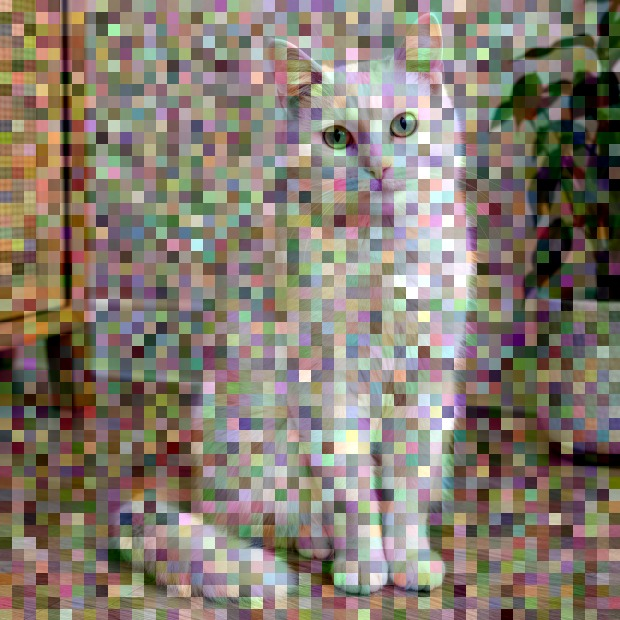
\includegraphics[width=1.35cm]{cat_noise2}};
\node[flowbox, minimum width=1.6cm, minimum height=0.9cm] (d2) at (5.9,0) {去噪};
\node[flowlab] at (7.75,0) {$\cdots$};
\node[thumb] (s0) at (10.0,0) {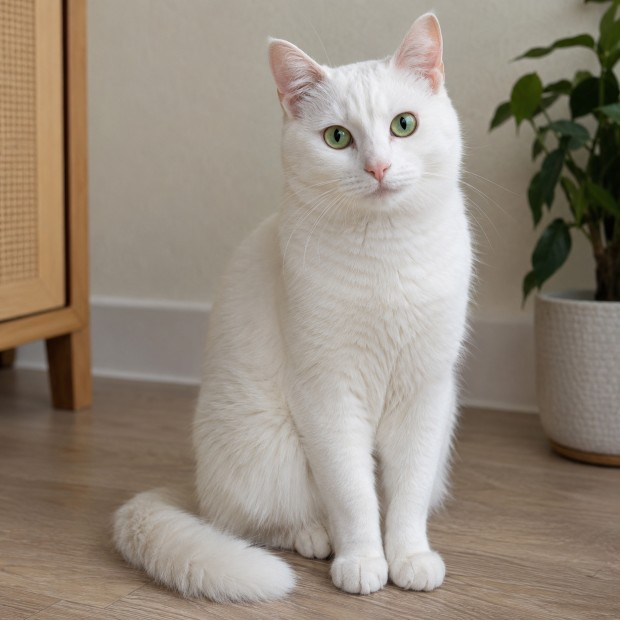
\includegraphics[width=1.35cm]{cat_white}};
\draw[flowarr] ($(sT.east)+(0.04,0)$) -- ($(d1.west)+(-0.04,0)$);
\draw[flowarr] ($(d1.east)+(0.04,0)$) -- ($(sT1.west)+(-0.04,0)$);
\draw[flowarr] ($(sT1.east)+(0.04,0)$) -- ($(d2.west)+(-0.04,0)$);
\draw[flowarr] ($(d2.east)+(0.04,0)$) -- (7.4,0);
\draw[flowarr] (8.1,0) -- ($(s0.west)+(-0.04,0)$);
\node[flowlab, below=3pt of sT] {$\bm{x}_T$};
\node[flowlab, below=3pt of sT1] {$\bm{x}_{T-1}$};
\node[flowlab, below=3pt of s0] {$\bm{x}_0$};
% ---- 放大指示：两条竖直虚线引向下方的虚线框 ----
\draw[dashed, gray!70] (3.28,-0.7) -- (3.28,-2.0);
\draw[dashed, gray!70] (4.62,-0.7) -- (4.62,-2.0);
\node[flowlab, text=black!70, anchor=west] at (4.85,-1.4) {放大其中一步};
% ---- 下排：虚线放大框 ----
\draw[dashed, gray!70, rounded corners=8pt] (-1.05,-2.0) rectangle (9.85,-5.45);
\node[thumb] (st) at (0,-2.9) {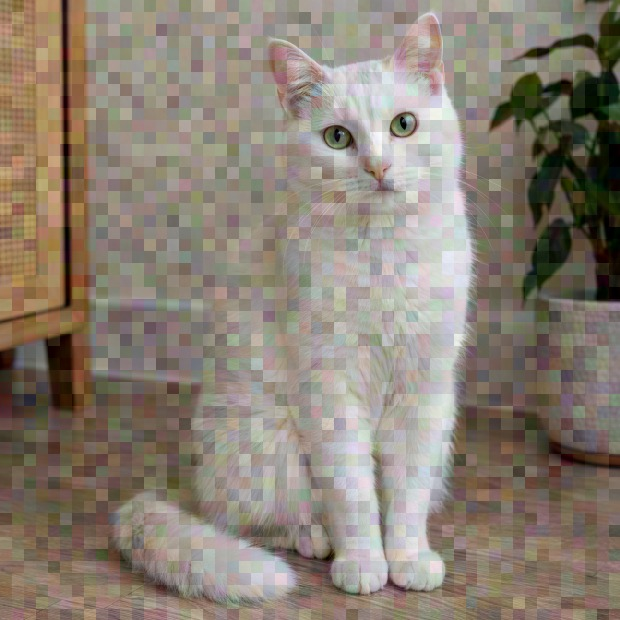
\includegraphics[width=1.35cm]{cat_noise1}};
\node[flowbox, minimum width=2.4cm, minimum height=1.0cm] (net) at (2.4,-2.9)
  {网络预测噪声\\$\bm{\epsilon}_\theta(\bm{x}_t,t)$};
\node[flowbox, minimum width=2.4cm, minimum height=1.0cm] (mu) at (5.5,-2.9)
  {算出均值 $\bm{\mu}_\theta$\\采样得 $\bm{x}_{t-1}$};
\node[thumb] (out) at (8.6,-2.9) {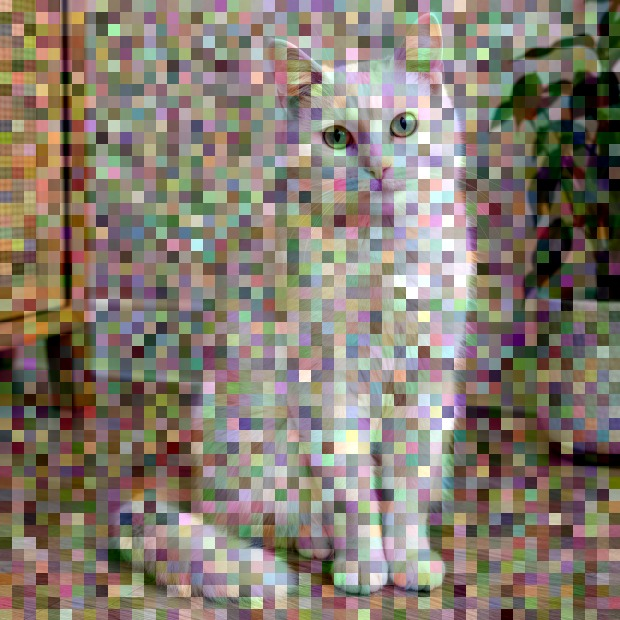
\includegraphics[width=1.35cm]{cat_noise2}};
\draw[flowarr] ($(st.east)+(0.04,0)$) -- ($(net.west)+(-0.04,0)$);
\draw[flowarr] ($(net.east)+(0.04,0)$) -- ($(mu.west)+(-0.04,0)$);
\draw[flowarr] ($(mu.east)+(0.04,0)$) -- ($(out.west)+(-0.04,0)$);
\node[flowlab, below=3pt of st] {$\bm{x}_t$};
\node[flowlab, below=3pt of out] {$\bm{x}_{t-1}$};
% ---- 框内公式 ----
\node[font=\small, align=center] at (4.3,-4.05)
  {$p_\theta(\bm{x}_{t-1}\mid\bm{x}_t)
    =\mathcal{N}\!\left(\bm{\mu}_\theta(\bm{x}_t,t),\,\sigma_t^2\bm{I}\right)$};
\node[font=\small, align=center] at (4.3,-4.85)
  {$\bm{\mu}_\theta=\dfrac{1}{\sqrt{\alpha_t}}
    \Bigl(\bm{x}_t-\dfrac{1-\alpha_t}{\sqrt{1-\bar{\alpha}_t}}\,
    \bm{\epsilon}_\theta(\bm{x}_t,t)\Bigr)$};
\end{tikzpicture}
\caption{反向计算框架}
\label{fig:framework}
\end{figure}

顺带回答一个常见疑问：为什么不直接让网络预测 $\bm{x}_0$？由式~\eqref{eq:4.7}，两种做法只差一个确定的线性变换，数学上等价；但噪声的取值范围稳定、作为回归目标更好训练，所以实践中更常用预测噪声。

\subsection{采样循环}

把前面的结果合起来，采样就是一个很短的循环。此时手里已经齐了：网络给出单步反向分布 $p_\theta(\bm{x}_{t-1}\mid\bm{x}_t)=\mathcal{N}(\bm{\mu}_\theta,\sigma_t^2\bm{I})$，均值按式~\eqref{eq:4.8} 由噪声预测 $\bm{\epsilon}_\theta$ 算出。于是从纯噪声出发，反复“预测噪声、去掉一部分、往前走一步”即可：

\begin{enumerate}
\item 从标准高斯分布采出起点 $\bm{x}_T\sim\mathcal{N}(\bm{0},\bm{I})$，令 $t=T$；
\item 把当前的 $\bm{x}_t$ 和时间步 $t$ 喂给网络，得到噪声预测 $\bm{\epsilon}_\theta(\bm{x}_t,t)$；
\item 代入式~\eqref{eq:4.9} 算出噪声更少一步的 $\bm{x}_{t-1}$，随后令 $t\leftarrow t-1$；
\item 重复前两步；当 $t=1$ 时不再加式~\eqref{eq:4.9} 末尾的随机项，算出的就是最终结果 $\bm{x}_0$。
\end{enumerate}
整个流程如图~\ref{fig:loop} 所示。

\begin{figure}[htbp]
\centering
\begin{tikzpicture}[x=1cm,y=1cm]
\node[flowbox, minimum width=2.6cm, minimum height=1.0cm] (net) at (0,0)
  {噪声预测网络\\$\bm{\epsilon}_\theta(\bm{x}_t,t)$};
\node[flowbox, minimum width=2.6cm, minimum height=1.0cm] (step) at (4.6,0)
  {按式~\eqref{eq:4.9}\\一步去噪};
\node[flowlab] at (-3.6,0) {输入};
\node[flowlab] at (-2.35,0) {$\bm{x}_t$};
\node[flowlab] at (7.35,0) {$\bm{x}_{t-1}$};
\draw[flowarr] (-1.8,0) -- ($(net.west)+(-0.04,0)$);
\draw[flowarr] ($(net.east)+(0.04,0)$) -- node[above,font=\small]{预测噪声} ($(step.west)+(-0.04,0)$);
\draw[flowarr] ($(step.east)+(0.04,0)$) -- node[above,font=\small]{去噪} (7.0,0);
\draw[flowarr] ($(step.north)+(0,0.05)$) .. controls +(0,1.05) and +(0,1.05) ..
  node[midway,above,font=\small]{令 $t\leftarrow t-1$，重复直到得到 $\bm{x}_0$} ($(net.north)+(0,0.05)$);
\end{tikzpicture}
\caption{采样循环}
\label{fig:loop}
\end{figure}

要注意，这个循环里既没有真实图片，也没有任何“对照答案”的步骤：每一步能用的信息只有当前的带噪样本 $\bm{x}_t$ 和时间步 $t$，模型全靠训练时学到的那点经验去判断“这张图被加了多少噪声”。

最后把视角拉远，看整条生成链在概率上意味着什么（图~\ref{fig:compute}）：上排是从 $\bm{x}_T$ 到 $\bm{x}_0$ 的完整采样链，每走一步都从单步反向分布里采一个样本；下排放大其中一步——网络去噪后给出这一步高斯分布的均值 $\bm{\mu}_\theta(\bm{x}_t,t)$，采出的 $\bm{x}_{t-1}$ 应当贴近这个均值。把链上每一步的概率连乘起来、对所有中间状态积分，就得到模型赋予一张完整图片的概率 $p_\theta(\bm{x}_0)$——它正是第~5 章训练目标想要最大化的对象。

\begin{figure}[htbp]
\centering
\begin{tikzpicture}[x=1cm,y=1cm,scale=0.9,transform shape]
% ---- 上排：完整采样链 ----
\node[thumb] (xT) at (0,0) {
\includegraphics[width=1.5cm]{noise_gray}};
\node[flowbox, minimum width=1.7cm, minimum height=0.9cm] (d1) at (2.2,0) {去噪};
\node[thumb] (xT1) at (4.4,0) {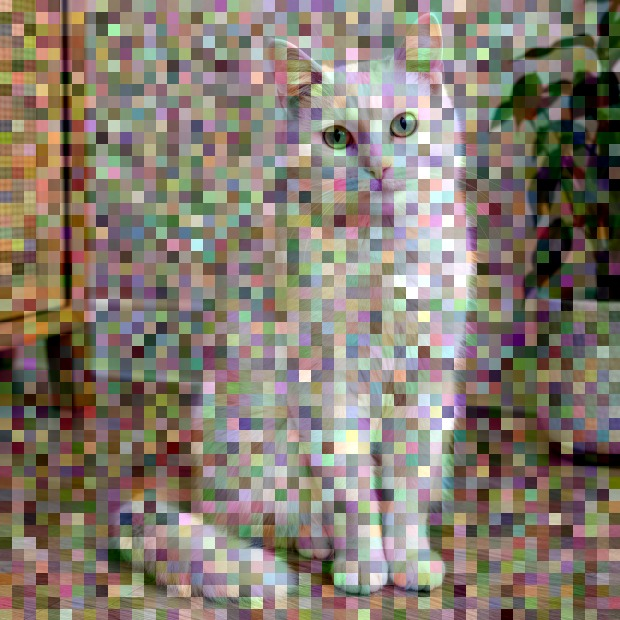
\includegraphics[width=1.5cm]{cat_noise2}};
\node[flowbox, minimum width=1.7cm, minimum height=0.9cm] (d2) at (6.6,0) {去噪};
\node[flowlab] at (8.5,0) {$\cdots$};
\node[thumb] (x0) at (10.4,0) {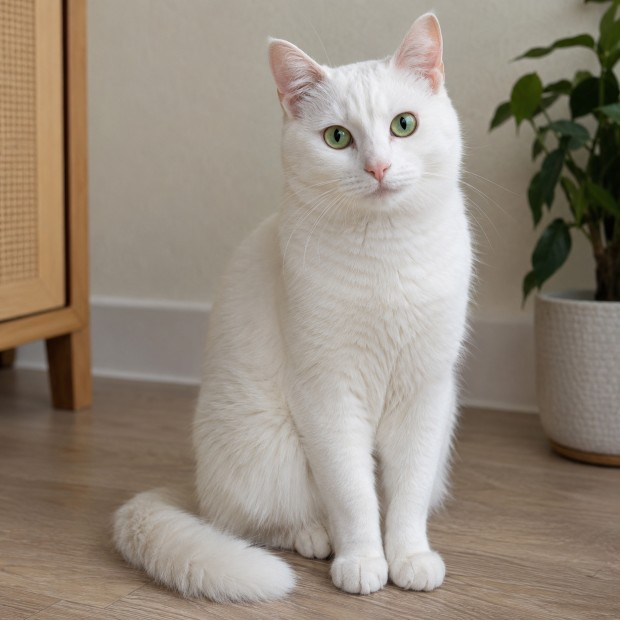
\includegraphics[width=1.5cm]{cat_white}};
\draw[flowarr] ($(xT.east)+(0.04,0)$) -- ($(d1.west)+(-0.04,0)$);
\draw[flowarr] ($(d1.east)+(0.04,0)$) -- ($(xT1.west)+(-0.04,0)$);
\draw[flowarr] ($(xT1.east)+(0.04,0)$) -- ($(d2.west)+(-0.04,0)$);
\draw[flowarr] ($(d2.east)+(0.04,0)$) -- (8.15,0);
\draw[flowarr] (8.85,0) -- ($(x0.west)+(-0.04,0)$);
\node[flowlab, below=3pt of xT] {$\bm{x}_T$};
\node[flowlab, below=3pt of xT1] {$\bm{x}_{T-1}$};
\node[flowlab, below=3pt of x0] {$\bm{x}_0$};
% ---- 下排：放大一步，网络输出均值 ----
\node[thumb] (xt) at (0,-2.7) {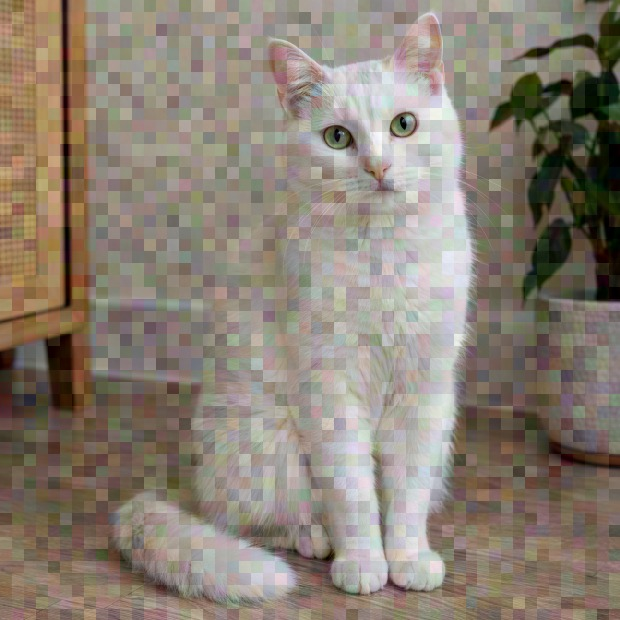
\includegraphics[width=1.5cm]{cat_noise1}};
\node[flowbox, minimum width=1.7cm, minimum height=0.9cm] (d3) at (2.2,-2.7) {去噪};
\node[flowbox, fill=blue!14, minimum width=2.1cm, minimum height=1.0cm] (g) at (5.1,-2.7)
  {$\bm{\mu}_\theta(\bm{x}_t,t)$};
\node[flowlab, below=2pt of g] {高斯均值};
\draw[flowarr] ($(xt.east)+(0.04,0)$) -- ($(d3.west)+(-0.04,0)$);
\draw[flowarr] ($(d3.east)+(0.04,0)$) -- ($(g.west)+(-0.04,0)$);
\node[flowlab, below=3pt of xt] {$\bm{x}_t$};
% ---- 右侧公式 ----
\node[anchor=west, font=\small] at (6.6,-2.7)
  {$p_\theta(\bm{x}_{t-1}\mid\bm{x}_t)
    =\mathcal{N}\!\left(\bm{\mu}_\theta(\bm{x}_t,t),\,\sigma_t^2\bm{I}\right)$};
% ---- 底部：连乘积分 ----
\node[font=\small, anchor=north] at (5.2,-4.1)
  {$p_\theta(\bm{x}_0)=\displaystyle\int p(\bm{x}_T)\,
    p_\theta(\bm{x}_{T-1}\mid\bm{x}_T)\cdots
    p_\theta(\bm{x}_{t-1}\mid\bm{x}_t)\cdots
    p_\theta(\bm{x}_0\mid\bm{x}_1)\,\mathrm{d}\bm{x}_{1:T}$};
\end{tikzpicture}
\caption{生成全景}
\label{fig:compute}
\end{figure}

\section{训练目标}

训练时，先从数据集中取出真实样本 $\bm{x}_0$，随机采样时间步 $t$ 和高斯噪声 $\bm{\epsilon}$，再利用公式~\eqref{eq:3.8} 构造带噪样本 $\bm{x}_t$。网络接收 $\bm{x}_t$ 和时间步 $t$，输出噪声预测 $\bm{\epsilon}_\theta(\bm{x}_t,t)$。

最常用的简化训练目标是噪声预测的均方误差：
\begin{equation}\label{eq:5.1}
\mathcal{L}_{\mathrm{simple}}
=\mathbb{E}_{\bm{x}_0,t,\bm{\epsilon}}
\left[\left\|\bm{\epsilon}-\bm{\epsilon}_\theta(\bm{x}_t,t)\right\|_2^2\right].
\end{equation}

\subsection{损失来源}

$\mathcal{L}_{\mathrm{simple}}$ 并不是拍脑袋选的，它来自对似然下界（ELBO）的推导。我们真正想要的是让模型给出真实图片的概率尽量大，即最大化 $\log p_\theta(\bm{x}_0)$；但 $p_\theta(\bm{x}_0)=\int p_\theta(\bm{x}_{0:T})\,\mathrm{d}\bm{x}_{1:T}$ 这个积分算不动，于是转而最大化它的下界：
\begin{equation}\label{eq:5.2}
\log p_\theta(\bm{x}_0)\;\ge\;
\mathbb{E}_{q(\bm{x}_{1:T}\mid\bm{x}_0)}
\!\left[\log\frac{p_\theta(\bm{x}_{0:T})}{q(\bm{x}_{1:T}\mid\bm{x}_0)}\right],
\end{equation}
其中联合分布 $p_\theta(\bm{x}_{0:T})=p(\bm{x}_T)\prod_{t=1}^{T}p_\theta(\bm{x}_{t-1}\mid\bm{x}_t)$ 就是反向链搭出来的整个生成过程。从下界到三项分解只有两步代数：先把分子分母沿马尔可夫链逐项展开，$t=1$ 的两项合在一起，正是“由 $\bm{x}_1$ 还原 $\bm{x}_0$”的重建期望；再对 $t\ge2$ 的每一项用贝叶斯公式
$q(\bm{x}_t\mid\bm{x}_{t-1})=q(\bm{x}_t\mid\bm{x}_0)\,q(\bm{x}_{t-1}\mid\bm{x}_t,\bm{x}_0)/q(\bm{x}_{t-1}\mid\bm{x}_0)$
改写，其中的 $q(\bm{x}_t\mid\bm{x}_0)$ 在相邻项之间首尾相消，剩下的项按“含 $p_\theta$ 的、含先验 $p(\bm{x}_T)$ 的、其余”归成三组，下界就拆成三块：
\begin{align}
\log p_\theta(\bm{x}_0)\;\ge\;&
\underbrace{\mathbb{E}_q\!\left[\log p_\theta(\bm{x}_0\mid\bm{x}_1)\right]}_{\text{重建项}}
-\underbrace{D_{\mathrm{KL}}\!\left(q(\bm{x}_T\mid\bm{x}_0)\,\big\|\,p(\bm{x}_T)\right)}_{\text{先验匹配项}}\notag\\[-2pt]
&-\sum_{t=2}^{T}
\underbrace{\mathbb{E}_q\!\left[D_{\mathrm{KL}}\!\left(
q(\bm{x}_{t-1}\mid\bm{x}_t,\bm{x}_0)\,\big\|\,p_\theta(\bm{x}_{t-1}\mid\bm{x}_t)
\right)\right]}_{\text{去噪匹配项}} .
\label{eq:5.3}
\end{align}
三项的含义：重建项要求 $\bm{x}_1$ 还能还原出 $\bm{x}_0$；先验匹配项要求加满噪声的 $\bm{x}_T$ 贴合标准高斯先验，这一项不含任何参数，是常数；真正训练网络的是去噪匹配项——每一步都在逼 $p_\theta(\bm{x}_{t-1}\mid\bm{x}_t)$ 去贴合 4.2 节推出的后验。两个分布都是方差固定的高斯，KL 散度只取决于均值之差，而 $p_\theta$ 的均值按式~\eqref{eq:4.8} 的形式由 $\bm{\epsilon}_\theta$ 给出、$q$ 的均值就是把 $\bm{\epsilon}_\theta$ 换成真值 $\bm{\epsilon}$，于是每一项展开后恰是 $\|\bm{\epsilon}-\bm{\epsilon}_\theta\|_2^2$（相差一些与网络无关的权重系数）。略去权重、把 $t$ 换成随机采样，就得到 $\mathcal{L}_{\mathrm{simple}}$——“预测噪声+均方误差”是 ELBO 逐项推导自然落下的结果，而非经验拼凑。

这个训练过程可以概括为：真实噪声是监督信号，带噪样本是输入，网络需要学会判断当前样本在当前噪声等级下被加入了什么噪声。训练完成后，模型便可以在没有真实样本的情况下，根据自己的噪声预测逐步采样。

\begin{itemize}
\item 输入：带噪样本 $\bm{x}_t$ 与时间步 $t$；
\item 监督信号：构造 $\bm{x}_t$ 时实际加入的噪声 $\bm{\epsilon}$；
\item 输出：模型预测的噪声 $\bm{\epsilon}_\theta(\bm{x}_t,t)$；
\item 损失：预测噪声与真实噪声之间的均方误差。
\end{itemize}

上述训练流程如图~\ref{fig:train} 所示。

\begin{figure}[htbp]
\centering
\begin{tikzpicture}[x=1cm,y=1cm]
\node[flowbox, minimum width=2.6cm, minimum height=1.0cm] (s0) at (0,0)
  {取出训练样本\\$\bm{x}_0$};
\node[flowbox, minimum width=3.1cm, minimum height=1.0cm] (sample) at (4.3,0)
  {随机采样\\$t$ 与 $\bm{\epsilon}\sim\mathcal{N}(\bm{0},\bm{I})$};
\node[flowbox, minimum width=2.6cm, minimum height=1.0cm] (xt) at (8.6,0)
  {由式~\eqref{eq:3.8}\\构造 $\bm{x}_t$};
\node[flowbox, minimum width=3.3cm, minimum height=1.0cm] (loss) at (1.9,-2.2)
  {计算损失\\$\|\bm{\epsilon}-\bm{\epsilon}_\theta(\bm{x}_t,t)\|_2^2$};
\node[flowbox, minimum width=2.6cm, minimum height=1.0cm] (net) at (6.3,-2.2)
  {网络预测\\$\bm{\epsilon}_\theta(\bm{x}_t,t)$};
\draw[flowarr] ($(s0.east)+(0.04,0)$) -- ($(sample.west)+(-0.04,0)$);
\draw[flowarr] ($(sample.east)+(0.04,0)$) -- ($(xt.west)+(-0.04,0)$);
\draw[flowarr] ($(xt.south)+(0,-0.04)$) -- node[pos=0.4, right=2pt, font=\small]{带噪样本 $\bm{x}_t$}
  ($(net.north)+(0,0.04)$);
\draw[flowarr] ($(sample.south)+(0,-0.04)$) .. controls +(-0.4,-0.5) and +(0.7,0) ..
  node[midway, above=1pt, font=\small]{真实噪声 $\bm{\epsilon}$（监督信号）}
  ($(loss.north)+(0.7,0.04)$);
\draw[flowarr] ($(net.west)+(-0.04,0)$) -- ($(loss.east)+(0.04,0)$);
\draw[dashed, gray!80, flowarr] ($(loss.south)+(0.4,0.04)$) .. controls +(0,-0.7) and +(0,-0.7) ..
  node[midway, below, font=\small]{反向传播，更新参数 $\theta$} ($(net.south)+(-0.4,0.04)$);
\end{tikzpicture}
\caption{训练流程}
\label{fig:train}
\end{figure}

\section{网络结构}

实际的噪声预测网络通常采用 U-Net 一类的结构，并通过时间嵌入把时间步 $t$ 提供给网络。对于条件生成，还可以把类别、文字等条件编码后注入网络，结构示意见图~\ref{fig:unet}。

\begin{figure}[htbp]
\centering
\begin{tikzpicture}[x=1cm,y=1cm]
\node[flowbox, minimum width=2.5cm, minimum height=1.0cm] (in) at (0,1.5)
  {输入 $\bm{x}_t$\\卷积块};
\node[flowbox, minimum width=2.5cm, minimum height=1.0cm] (out) at (7.6,1.5)
  {卷积块\\输出 $\hat{\bm{\epsilon}}$};
\draw[flowarr] ($(in.east)+(0.05,0)$) -- node[above,font=\small]{跳跃连接（保留细节）} ($(out.west)+(-0.05,0)$);
\node[flowbox, minimum width=2.5cm, minimum height=1.0cm] (down) at (0,-0.3)
  {下采样\\卷积块};
\node[flowbox, minimum width=2.5cm, minimum height=1.0cm] (up) at (7.6,-0.3)
  {上采样\\卷积块};
\draw[flowarr] ($(in.south)+(0,-0.04)$) -- ($(down.north)+(0,0.04)$);
\draw[flowarr] ($(up.north)+(0,0.04)$) -- ($(out.south)+(0,-0.04)$);
\node[flowbox, minimum width=2.2cm, minimum height=0.85cm] (bot) at (3.8,-1.95)
  {瓶颈层};
\draw[flowarr] ($(down.south)+(0,-0.04)$) .. controls +(0,-1.0) and +(-2.6,0) .. ($(bot.west)+(-0.04,0)$);
\draw[flowarr] ($(bot.east)+(0.04,0)$) .. controls +(2.6,0) and +(0,-1.0) .. ($(up.south)+(0,-0.04)$);
\node[fill=orange!12, draw=orange!60!black, rounded corners=4pt, inner sep=4pt,
      minimum width=5.4cm, minimum height=1.0cm, align=center, font=\small] (te) at (3.8,-3.6)
  {时间嵌入：$t$ 的正弦编码\\（也可同时注入类别 / 文本条件）};
\draw[flowarr] ($(te.north)+(0,0.04)$) -- ($(bot.south)+(0,-0.04)$);
\draw[gray!80, dashed, flowarr] ($(down.east)+(0.15,0)$) -- ($(up.west)+(-0.15,0)$);
\end{tikzpicture}
\caption{网络结构}
\label{fig:unet}
\end{figure}

U-Net 的分工可以这样理解：下采样路径把图片逐步压缩，让网络在低分辨率上看到整张图的全局结构（噪声大概加在哪、整体布局是什么）；上采样路径再把分辨率逐步恢复回来；两路之间的跳跃连接把编码阶段保留的细节直接送进解码阶段，所以输出既能去噪、又不丢纹理。时间嵌入解决的是“同一个网络怎么区分不同噪声等级”的问题：$t$ 先经过正弦编码变成一个向量，再注入每个残差块，相当于告诉网络“当前是加了 $t$ 步噪声的版本，该减多少噪声”。做条件生成时，类别或文本编码也走这条注入通道，网络就能按条件往指定的方向去噪。

\end{document}
